
%% bare_jrnl_comsoc.tex
%% V1.4b
%% 2015/08/26
%% by Michael Shell
%% see http://www.michaelshell.org/
%% for current contact information.
%%
%% This is a skeleton file demonstrating the use of IEEEtran.cls
%% (requires IEEEtran.cls version 1.8b or later) with an IEEE
%% Communications Society journal paper.
%%
%% Support sites:
%% http://www.michaelshell.org/tex/ieeetran/
%% http://www.ctan.org/pkg/ieeetran
%% and
%% http://www.ieee.org/

%%*************************************************************************
%% Legal Notice:
%% This code is offered as-is without any warranty either expressed or
%% implied; without even the implied warranty of MERCHANTABILITY or
%% FITNESS FOR A PARTICULAR PURPOSE! 
%% User assumes all risk.
%% In no event shall the IEEE or any contributor to this code be liable for
%% any damages or losses, including, but not limited to, incidental,
%% consequential, or any other damages, resulting from the use or misuse
%% of any information contained here.
%%
%% All comments are the opinions of their respective authors and are not
%% necessarily endorsed by the IEEE.
%%
%% This work is distributed under the LaTeX Project Public License (LPPL)
%% ( http://www.latex-project.org/ ) version 1.3, and may be freely used,
%% distributed and modified. A copy of the LPPL, version 1.3, is included
%% in the base LaTeX documentation of all distributions of LaTeX released
%% 2003/12/01 or later.
%% Retain all contribution notices and credits.
%% ** Modified files should be clearly indicated as such, including  **
%% ** renaming them and changing author support contact information. **
%%*************************************************************************


% *** Authors should verify (and, if needed, correct) their LaTeX system  ***
% *** with the testflow diagnostic prior to trusting their LaTeX platform ***
% *** with production work. The IEEE's font choices and paper sizes can   ***
% *** trigger bugs that do not appear when using other class files.       ***                          ***
% The testflow support page is at:
% http://www.michaelshell.org/tex/testflow/



\documentclass[conference,comsoc]{IEEEtran}
%
% If IEEEtran.cls has not been installed into the LaTeX system files,
% manually specify the path to it like:
% \documentclass[journal,comsoc]{../sty/IEEEtran}


\usepackage[T1]{fontenc}% optional T1 font encoding


% Some very useful LaTeX packages include:
% (uncomment the ones you want to load)


% *** MISC UTILITY PACKAGES ***
%
%\usepackage{ifpdf}
% Heiko Oberdiek's ifpdf.sty is very useful if you need conditional
% compilation based on whether the output is pdf or dvi.
% usage:
% \ifpdf
%   % pdf code
% \else
%   % dvi code
% \fi
% The latest version of ifpdf.sty can be obtained from:
% http://www.ctan.org/pkg/ifpdf
% Also, note that IEEEtran.cls V1.7 and later provides a builtin
% \ifCLASSINFOpdf conditional that works the same way.
% When switching from latex to pdflatex and vice-versa, the compiler may
% have to be run twice to clear warning/error messages.






% *** CITATION PACKAGES ***
%
%\usepackage{cite}
% cite.sty was written by Donald Arseneau
% V1.6 and later of IEEEtran pre-defines the format of the cite.sty package
% \cite{} output to follow that of the IEEE. Loading the cite package will
% result in citation numbers being automatically sorted and properly
% "compressed/ranged". e.g., [1], [9], [2], [7], [5], [6] without using
% cite.sty will become [1], [2], [5]--[7], [9] using cite.sty. cite.sty's
% \cite will automatically add leading space, if needed. Use cite.sty's
% noadjust option (cite.sty V3.8 and later) if you want to turn this off
% such as if a citation ever needs to be enclosed in parenthesis.
% cite.sty is already installed on most LaTeX systems. Be sure and use
% version 5.0 (2009-03-20) and later if using hyperref.sty.
% The latest version can be obtained at:
% http://www.ctan.org/pkg/cite
% The documentation is contained in the cite.sty file itself.






% *** GRAPHICS RELATED PACKAGES ***
%
\ifCLASSINFOpdf
  % \usepackage[pdftex]{graphicx}
  % declare the path(s) where your graphic files are
  % \graphicspath{{../pdf/}{../jpeg/}}
  % and their extensions so you won't have to specify these with
  % every instance of \includegraphics
  % \DeclareGraphicsExtensions{.pdf,.jpeg,.png}
\else
  % or other class option (dvipsone, dvipdf, if not using dvips). graphicx
  % will default to the driver specified in the system graphics.cfg if no
  % driver is specified.
  % \usepackage[dvips]{graphicx}
  % declare the path(s) where your graphic files are
  % \graphicspath{{../eps/}}
  % and their extensions so you won't have to specify these with
  % every instance of \includegraphics
  % \DeclareGraphicsExtensions{.eps}
\fi
% graphicx was written by David Carlisle and Sebastian Rahtz. It is
% required if you want graphics, photos, etc. graphicx.sty is already
% installed on most LaTeX systems. The latest version and documentation
% can be obtained at: 
% http://www.ctan.org/pkg/graphicx
% Another good source of documentation is "Using Imported Graphics in
% LaTeX2e" by Keith Reckdahl which can be found at:
% http://www.ctan.org/pkg/epslatex
%
% latex, and pdflatex in dvi mode, support graphics in encapsulated
% postscript (.eps) format. pdflatex in pdf mode supports graphics
% in .pdf, .jpeg, .png and .mps (metapost) formats. Users should ensure
% that all non-photo figures use a vector format (.eps, .pdf, .mps) and
% not a bitmapped formats (.jpeg, .png). The IEEE frowns on bitmapped formats
% which can result in "jaggedy"/blurry rendering of lines and letters as
% well as large increases in file sizes.
%
% You can find documentation about the pdfTeX application at:
% http://www.tug.org/applications/pdftex





% *** MATH PACKAGES ***
%
\usepackage{amsmath}
% A popular package from the American Mathematical Society that provides
% many useful and powerful commands for dealing with mathematics.
% Do NOT use the amsbsy package under comsoc mode as that feature is
% already built into the Times Math font (newtxmath, mathtime, etc.).
% 
% Also, note that the amsmath package sets \interdisplaylinepenalty to 10000
% thus preventing page breaks from occurring within multiline equations. Use:
\interdisplaylinepenalty=2500
% after loading amsmath to restore such page breaks as IEEEtran.cls normally
% does. amsmath.sty is already installed on most LaTeX systems. The latest
% version and documentation can be obtained at:
% http://www.ctan.org/pkg/amsmath


% Select a Times math font under comsoc mode or else one will automatically
% be selected for you at the document start. This is required as Communications
% Society journals use a Times, not Computer Modern, math font.
\usepackage[cmintegrals]{newtxmath}
% The freely available newtxmath package was written by Michael Sharpe and
% provides a feature rich Times math font. The cmintegrals option, which is
% the default under IEEEtran, is needed to get the correct style integral
% symbols used in Communications Society journals. Version 1.451, July 28,
% 2015 or later is recommended. Also, do *not* load the newtxtext.sty package
% as doing so would alter the main text font.
% http://www.ctan.org/pkg/newtx
%
% Alternatively, you can use the MathTime commercial fonts if you have them
% installed on your system:
%\usepackage{mtpro2}
%\usepackage{mt11p}
%\usepackage{mathtime}


%\usepackage{bm}
% The bm.sty package was written by David Carlisle and Frank Mittelbach.
% This package provides a \bm{} to produce bold math symbols.
% http://www.ctan.org/pkg/bm





% *** SPECIALIZED LIST PACKAGES ***
%
%\usepackage{algorithmic}
% algorithmic.sty was written by Peter Williams and Rogerio Brito.
% This package provides an algorithmic environment fo describing algorithms.
% You can use the algorithmic environment in-text or within a figure
% environment to provide for a floating algorithm. Do NOT use the algorithm
% floating environment provided by algorithm.sty (by the same authors) or
% algorithm2e.sty (by Christophe Fiorio) as the IEEE does not use dedicated
% algorithm float types and packages that provide these will not provide
% correct IEEE style captions. The latest version and documentation of
% algorithmic.sty can be obtained at:
% http://www.ctan.org/pkg/algorithms
% Also of interest may be the (relatively newer and more customizable)
% algorithmicx.sty package by Szasz Janos:
% http://www.ctan.org/pkg/algorithmicx




% *** ALIGNMENT PACKAGES ***
%
%\usepackage{array}
% Frank Mittelbach's and David Carlisle's array.sty patches and improves
% the standard LaTeX2e array and tabular environments to provide better
% appearance and additional user controls. As the default LaTeX2e table
% generation code is lacking to the point of almost being broken with
% respect to the quality of the end results, all users are strongly
% advised to use an enhanced (at the very least that provided by array.sty)
% set of table tools. array.sty is already installed on most systems. The
% latest version and documentation can be obtained at:
% http://www.ctan.org/pkg/array


% IEEEtran contains the IEEEeqnarray family of commands that can be used to
% generate multiline equations as well as matrices, tables, etc., of high
% quality.




% *** SUBFIGURE PACKAGES ***
%\ifCLASSOPTIONcompsoc
%  \usepackage[caption=false,font=normalsize,labelfont=sf,textfont=sf]{subfig}
%\else
%  \usepackage[caption=false,font=footnotesize]{subfig}
%\fi
% subfig.sty, written by Steven Douglas Cochran, is the modern replacement
% for subfigure.sty, the latter of which is no longer maintained and is
% incompatible with some LaTeX packages including fixltx2e. However,
% subfig.sty requires and automatically loads Axel Sommerfeldt's caption.sty
% which will override IEEEtran.cls' handling of captions and this will result
% in non-IEEE style figure/table captions. To prevent this problem, be sure
% and invoke subfig.sty's "caption=false" package option (available since
% subfig.sty version 1.3, 2005/06/28) as this is will preserve IEEEtran.cls
% handling of captions.
% Note that the Computer Society format requires a larger sans serif font
% than the serif footnote size font used in traditional IEEE formatting
% and thus the need to invoke different subfig.sty package options depending
% on whether compsoc mode has been enabled.
%
% The latest version and documentation of subfig.sty can be obtained at:
% http://www.ctan.org/pkg/subfig




% *** FLOAT PACKAGES ***
%
%\usepackage{fixltx2e}
% fixltx2e, the successor to the earlier fix2col.sty, was written by
% Frank Mittelbach and David Carlisle. This package corrects a few problems
% in the LaTeX2e kernel, the most notable of which is that in current
% LaTeX2e releases, the ordering of single and double column floats is not
% guaranteed to be preserved. Thus, an unpatched LaTeX2e can allow a
% single column figure to be placed prior to an earlier double column
% figure.
% Be aware that LaTeX2e kernels dated 2015 and later have fixltx2e.sty's
% corrections already built into the system in which case a warning will
% be issued if an attempt is made to load fixltx2e.sty as it is no longer
% needed.
% The latest version and documentation can be found at:
% http://www.ctan.org/pkg/fixltx2e


%\usepackage{stfloats}
% stfloats.sty was written by Sigitas Tolusis. This package gives LaTeX2e
% the ability to do double column floats at the bottom of the page as well
% as the top. (e.g., "\begin{figure*}[!b]" is not normally possible in
% LaTeX2e). It also provides a command:
%\fnbelowfloat
% to enable the placement of footnotes below bottom floats (the standard
% LaTeX2e kernel puts them above bottom floats). This is an invasive package
% which rewrites many portions of the LaTeX2e float routines. It may not work
% with other packages that modify the LaTeX2e float routines. The latest
% version and documentation can be obtained at:
% http://www.ctan.org/pkg/stfloats
% Do not use the stfloats baselinefloat ability as the IEEE does not allow
% \baselineskip to stretch. Authors submitting work to the IEEE should note
% that the IEEE rarely uses double column equations and that authors should try
% to avoid such use. Do not be tempted to use the cuted.sty or midfloat.sty
% packages (also by Sigitas Tolusis) as the IEEE does not format its papers in
% such ways.
% Do not attempt to use stfloats with fixltx2e as they are incompatible.
% Instead, use Morten Hogholm'a dblfloatfix which combines the features
% of both fixltx2e and stfloats:
%
% \usepackage{dblfloatfix}
% The latest version can be found at:
% http://www.ctan.org/pkg/dblfloatfix




%\ifCLASSOPTIONcaptionsoff
%  \usepackage[nomarkers]{endfloat}
% \let\MYoriglatexcaption\caption
% \renewcommand{\caption}[2][\relax]{\MYoriglatexcaption[#2]{#2}}
%\fi
% endfloat.sty was written by James Darrell McCauley, Jeff Goldberg and 
% Axel Sommerfeldt. This package may be useful when used in conjunction with 
% IEEEtran.cls'  captionsoff option. Some IEEE journals/societies require that
% submissions have lists of figures/tables at the end of the paper and that
% figures/tables without any captions are placed on a page by themselves at
% the end of the document. If needed, the draftcls IEEEtran class option or
% \CLASSINPUTbaselinestretch interface can be used to increase the line
% spacing as well. Be sure and use the nomarkers option of endfloat to
% prevent endfloat from "marking" where the figures would have been placed
% in the text. The two hack lines of code above are a slight modification of
% that suggested by in the endfloat docs (section 8.4.1) to ensure that
% the full captions always appear in the list of figures/tables - even if
% the user used the short optional argument of \caption[]{}.
% IEEE papers do not typically make use of \caption[]'s optional argument,
% so this should not be an issue. A similar trick can be used to disable
% captions of packages such as subfig.sty that lack options to turn off
% the subcaptions:
% For subfig.sty:
% \let\MYorigsubfloat\subfloat
% \renewcommand{\subfloat}[2][\relax]{\MYorigsubfloat[]{#2}}
% However, the above trick will not work if both optional arguments of
% the \subfloat command are used. Furthermore, there needs to be a
% description of each subfigure *somewhere* and endfloat does not add
% subfigure captions to its list of figures. Thus, the best approach is to
% avoid the use of subfigure captions (many IEEE journals avoid them anyway)
% and instead reference/explain all the subfigures within the main caption.
% The latest version of endfloat.sty and its documentation can obtained at:
% http://www.ctan.org/pkg/endfloat
%
% The IEEEtran \ifCLASSOPTIONcaptionsoff conditional can also be used
% later in the document, say, to conditionally put the References on a 
% page by themselves.




% *** PDF, URL AND HYPERLINK PACKAGES ***
%
%\usepackage{url}
% url.sty was written by Donald Arseneau. It provides better support for
% handling and breaking URLs. url.sty is already installed on most LaTeX
% systems. The latest version and documentation can be obtained at:
% http://www.ctan.org/pkg/url
% Basically, \url{my_url_here}.




% *** Do not adjust lengths that control margins, column widths, etc. ***
% *** Do not use packages that alter fonts (such as pslatex).         ***
% There should be no need to do such things with IEEEtran.cls V1.6 and later.
% (Unless specifically asked to do so by the journal or conference you plan
% to submit to, of course. )


% correct bad hyphenation here
\hyphenation{op-tical net-works semi-conduc-tor}

%package for graphs
\usepackage{pgfplots}

\begin{document}
%
% paper title
% Titles are generally capitalized except for words such as a, an, and, as,
% at, but, by, for, in, nor, of, on, or, the, to and up, which are usually
% not capitalized unless they are the first or last word of the title.
% Linebreaks \\ can be used within to get better formatting as desired.
% Do not put math or special symbols in the title.
\title{Comparison of Two CoAP Protocols for  Cloud Connecting Constrained Devices}
%
%
% author names and IEEE memberships
% note positions of commas and nonbreaking spaces ( ~ ) LaTeX will not break
% a structure at a ~ so this keeps an author's name from being broken across
% two lines.
% use \thanks{} to gain access to the first footnote area
% a separate \thanks must be used for each paragraph as LaTeX2e's \thanks
% was not built to handle multiple paragraphs
%

\author{Bilal~Kais,~\IEEEmembership{M.Sc.~Student,~Aarhus~University~Engineering Department,}
        and~Khaled~Saied,~\IEEEmembership{M.Sc.~Student,~Aarhus~University~Engineering Department}% <-this % stops a space
\thanks{M. Shell was with the Department
of Electrical and Computer Engineering, Georgia Institute of Technology, Atlanta,
GA, 30332 USA e-mail: (see http://www.michaelshell.org/contact.html).}% <-this % stops a space
\thanks{J. Doe and J. Doe are with Anonymous University.}% <-this % stops a space
\thanks{Manuscript received April 19, 2005; revised August 26, 2015.}}

% note the % following the last \IEEEmembership and also \thanks - 
% these prevent an unwanted space from occurring between the last author name
% and the end of the author line. i.e., if you had this:
% 
% \author{....lastname \thanks{...} \thanks{...} }
%                     ^------------^------------^----Do not want these spaces!
%
% a space would be appended to the last name and could cause every name on that
% line to be shifted left slightly. This is one of those "LaTeX things". For
% instance, "\textbf{A} \textbf{B}" will typeset as "A B" not "AB". To get
% "AB" then you have to do: "\textbf{A}\textbf{B}"
% \thanks is no different in this regard, so shield the last } of each \thanks
% that ends a line with a % and do not let a space in before the next \thanks.
% Spaces after \IEEEmembership other than the last one are OK (and needed) as
% you are supposed to have spaces between the names. For what it is worth,
% this is a minor point as most people would not even notice if the said evil
% space somehow managed to creep in.



% The paper headers
\markboth{Journal of \LaTeX\ Class Files,~Vol.~14, No.~8, August~2015}%
{Shell \MakeLowercase{\textit{et al.}}: Bare Demo of IEEEtran.cls for IEEE Communications Society Journals}
% The only time the second header will appear is for the odd numbered pages
% after the title page when using the twoside option.
% 
% *** Note that you probably will NOT want to include the author's ***
% *** name in the headers of peer review papers.                   ***
% You can use \ifCLASSOPTIONpeerreview for conditional compilation here if
% you desire.




% If you want to put a publisher's ID mark on the page you can do it like
% this:
%\IEEEpubid{0000--0000/00\$00.00~\copyright~2015 IEEE}
% Remember, if you use this you must call \IEEEpubidadjcol in the second
% column for its text to clear the IEEEpubid mark.



% use for special paper notices
%\IEEEspecialpapernotice{(Invited Paper)}




% make the title area
\maketitle

% As a general rule, do not put math, special symbols or citations
% in the abstract or keywords.
\begin{abstract}
Internet of Things (IoT) is expected to consist of billions of devices by 2020. Constrained devices are an essential part of IoT and therefore the focus is on developing lightweight protocols enabling, among others, cloud communication. CoAP, a lightweight web transfer protocol, is developed in recent years and is already in use. A new version of CoAP has been proposed which presents a modified CoAP that runs over TCP instead of UDP. IoTivity has used CoAP before and has recently published a new version with CoAP over TCP implemented, specifically for cloud communication. In this paper a comparison between CoAP and CoAP over TCP is made focusing on the energy consumption by analysing the bandwidth and latency. A concrete case is given with the use of Arduino Due using an Arduino WiFi Shield to exemplify the energy consumption of the two versions of CoAP in a constrained device.
The evaluation of the results shows ???.
\end{abstract}

% Note that keywords are not normally used for peerreview papers.
\begin{IEEEkeywords}
CoAP, CoAP over TCP, IoTivity, constrained devices, IoT, cloud, Arduino, UDP, TCP.
\end{IEEEkeywords}




% For peer review papers, you can put extra information on the cover
% page as needed:
% \ifCLASSOPTIONpeerreview
% \begin{center} \bfseries EDICS Category: 3-BBND \end{center}
% \fi
%
% For peerreview papers, this IEEEtran command inserts a page break and
% creates the second title. It will be ignored for other modes.
\IEEEpeerreviewmaketitle



%\section{Introduction}
\section{Introduction}
The Internet of Things (IoT) is one of the larger focus areas in today's research of newer computer 6technology. One definition for IoT is interconnection of computing devices embedded in everyday objects via the Internet, enabling them to send and receive data.

According to Cisco, the amount of interconnected devices will be 50 billion by 2020 \cite{ciscoiot:online} \cite{Inter74:online}.

\IEEEPARstart{C}{\MakeLowercase{onstrained}} devices are an essential part of IoT and therefore there is focus on developing lightweight protocols which enables different connectivity models for constrained devices.  
CoAP is one of the emerging lightweight application protocols which is designed for machine-to-machine (M2M) applications for use in constrained environments.   

Previously research has been done in the IoTivity framework which operates as a middleware trying to solve interoperability issues in the IoT \cite{interoperabilityChallenge}. Interoperability is about making IoT devices able to connect to any other device or system independent of the used technologies and exchange information as desired, and this area has if solved a potential great economic impact \cite{Unloc34:online}. 
Results from the research shows that IoTivity does not have the capability to communicate with the cloud in an appropriate way. 

IoTivity made use of the CoAP protocol as the only application protocol. 
A new version of the IoTivity framework has been published recently, where they have implemented a solution to connect IoT devices to the Cloud \cite{IoTiv3:online}. The solution was based on a newer draft for CoAP \cite{ietf-core-coap-tcp-tls-02} which presents a modified CoAP that runs over TCP instead of UDP.
The TCP protocol is more complex compared with the UDP protocol and thus it is in general more resource consuming \cite{giannoulis2009tcp}.
%it is in general not easy to employ on constrained devices. 

% More details from papers about tcp vs udp memory consumption

% Bilal har en ide som han ikke ønsker!
In this paper we will investigate if it is advantageous to use TCP as a transport protocol in CoAP instead of UDP when CoAP is used for constrained IoT devices. This investigation will be done by analysing the two versions of the CoAP protocol using a \textcolor{red}{qualitative method, where the focus is on significant architectural differences}, and a quantitative analytic method with focus on memory and energy consumption. 

The rest of this paper is structured as follows.  Section 2 presents the UDP and TCP versions of CoAP protocol. Section 3 provides a qualitative comparison. Section 4 provides a quantitative analytic comparison of the two protocols. Section 5 discusses the results and concludes the paper.     

\section{Background}

\subsection{Constrained Application Protocol}
CoAP is a lightweight web transfer protocol specialized for use with constrained devices and is currently a Proposed Standard RFC made by The Internet Engineering Task Force (IETF) \cite{Inter93:online}. CoAP is designed for M2M communication which includes the device-to-cloud connectivity model.
CoAP runs over the UDP transport protocol which helps keeping the message overhead small and thereby limits the need for fragmentation.
CoAP can be reliable even though UDP is used as transport protocol because CoAP handles the reliability and congestion control by enabling the message type Confirmable (CON). 
The use of confirmable message means that it requires an acknowledgement from the receiver of the message. 
To limit the number of simultaneous unacknowledged and confirmable messages, congestion control is implemented by use of the back-off algorithm.

The message format for CoAP, illustrated in \figurename{\ref{fig:msgformatcoap}}, contains among others a header with a length of 4 bytes. 
%a token for identifying the different requests, CoAP options, and payload. 
\begin{figure}[bht]
	\centering
	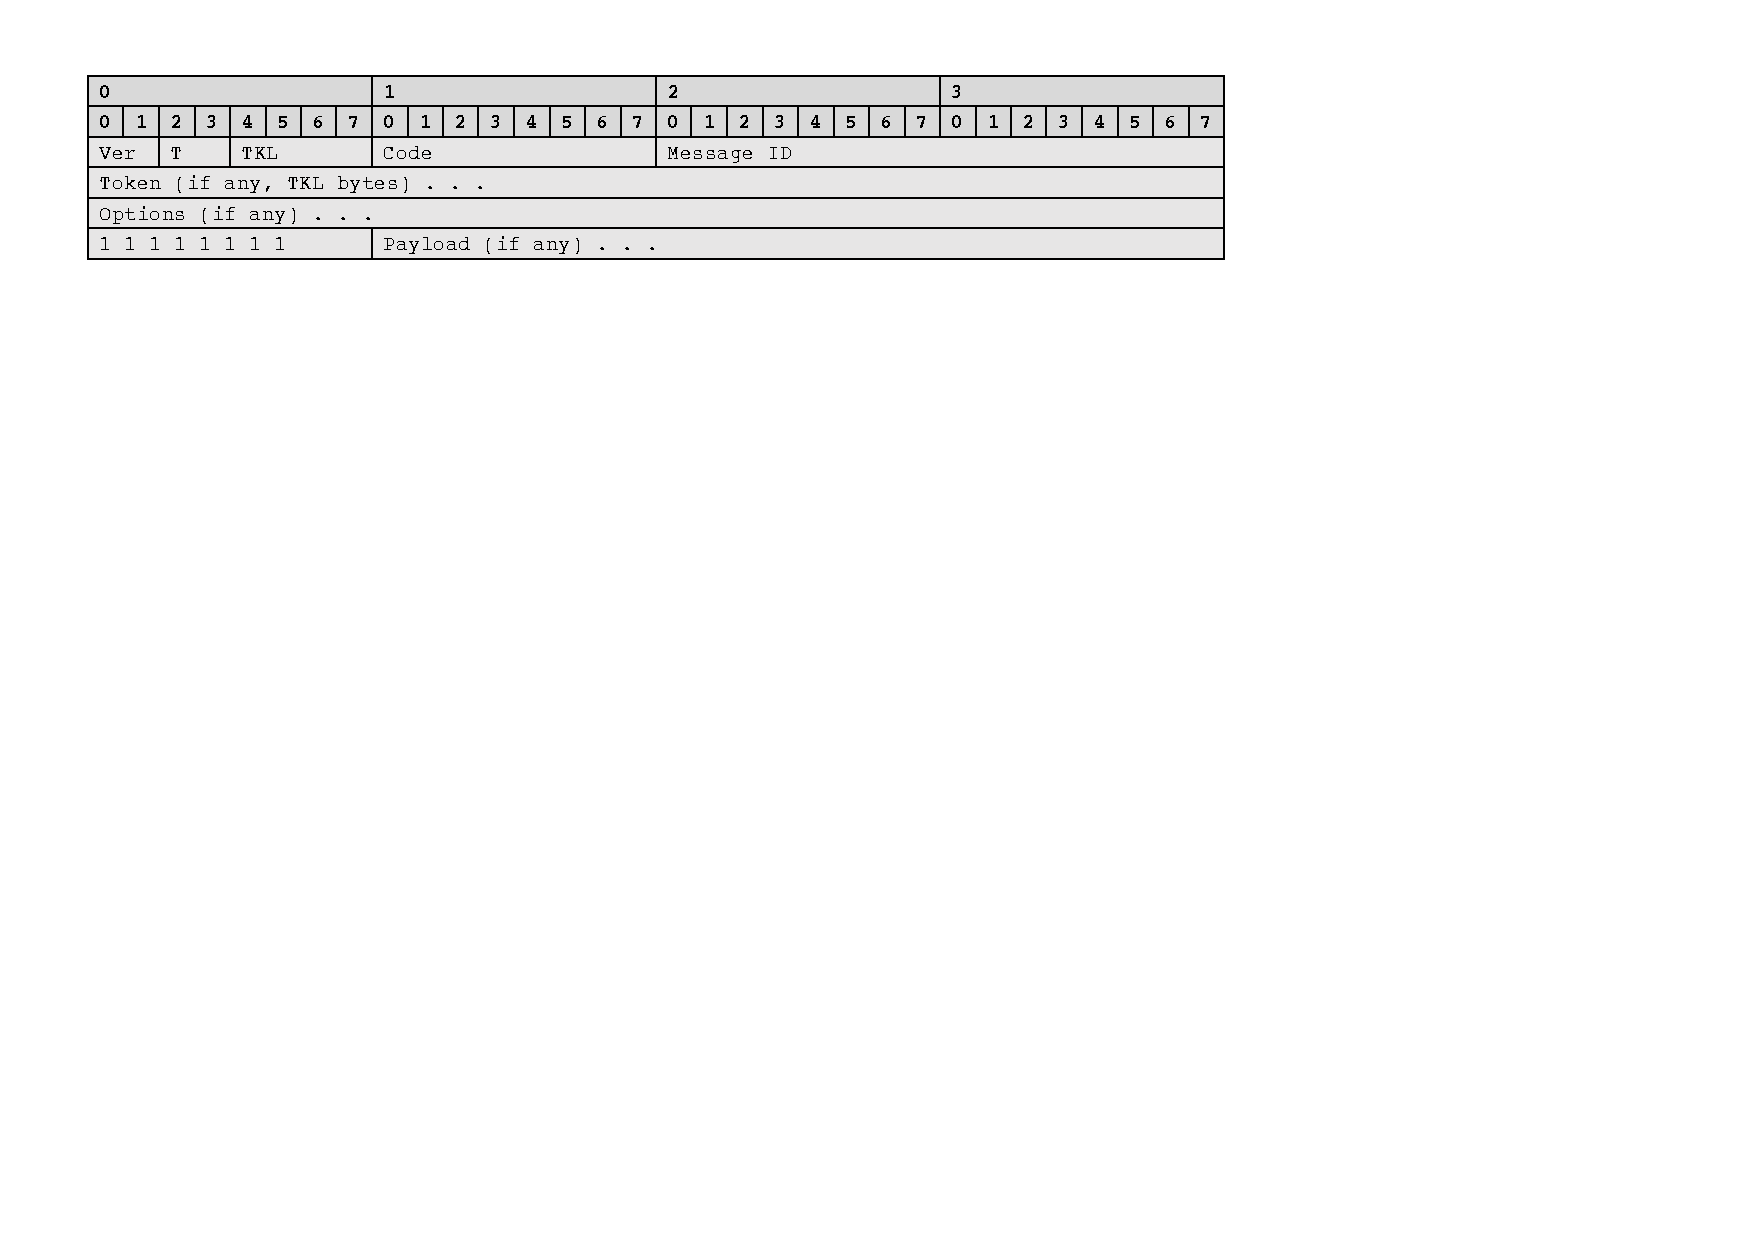
\includegraphics[width=3.5in]{gfx/msgformat-coap}
	\caption{The CoAP header.}
	\label{fig:msgformatcoap}
\end{figure}

The header contains following fields: 
\begin{list}{-}{}
	\item Version (ver) indicates the version of the CoAP protocol.
	\item Type (T) indicates the type of the message e.g. non-confirmable.
	\item Token length (TKL) indicates the length of Token field.
	\item Code indicates the status of the response or the request method. 
	\item Message ID is an identifier for relating acknowledgements to CON-messages and detection of duplicated messages as well.
\end{list}


%not asynchronous - has to wait for an aknowledged

%For security the Datagram Transport Layer Security (DTLS), which is based on the stream-oriented Transport Layer Security (TLS), is used.

%--UDP can only transfer small amounts of data

\subsection{Constrained Application Protocol over TCP}
CoAP over TCP is an Active Internet-Draft made by IETF. 
In this draft it is proposed to use TCP as a transport protocol instead of UDP.
CoAP over TCP is made for use for certain environments that benefits from using CoAP directly over a reliable communication channel which easily can come through firewalls, provides additional information to NAT, has longer session life, and is able to send requests asynchronously. 

CoAP over TCP is based on the original version of CoAP with some modifications. 
The use of TCP as a transport layer protocol removes the need for handling reliability, congestion control, and other features, which already exist in TCP, at the CoAP level.
Since it is not necessary to handle reliability at the CoAP level, all the communication in the CoAP over TCP are by use of non-confirmable (NON) messages and thereby the fields, Type (T) and Message ID, are unnecessary and thus removed from the header. 
The Message ID is also removed because TCP handles duplication detection as well.
Moreover the version (ver) is also removed from the header. The reason for this change is not specified in the draft.

Two new fields are added to the CoAP over TCP header as illustrated in \figurename{\ref{fig:msgformatcoapovertcp}}.
\begin{figure}[bht]
	\centering
	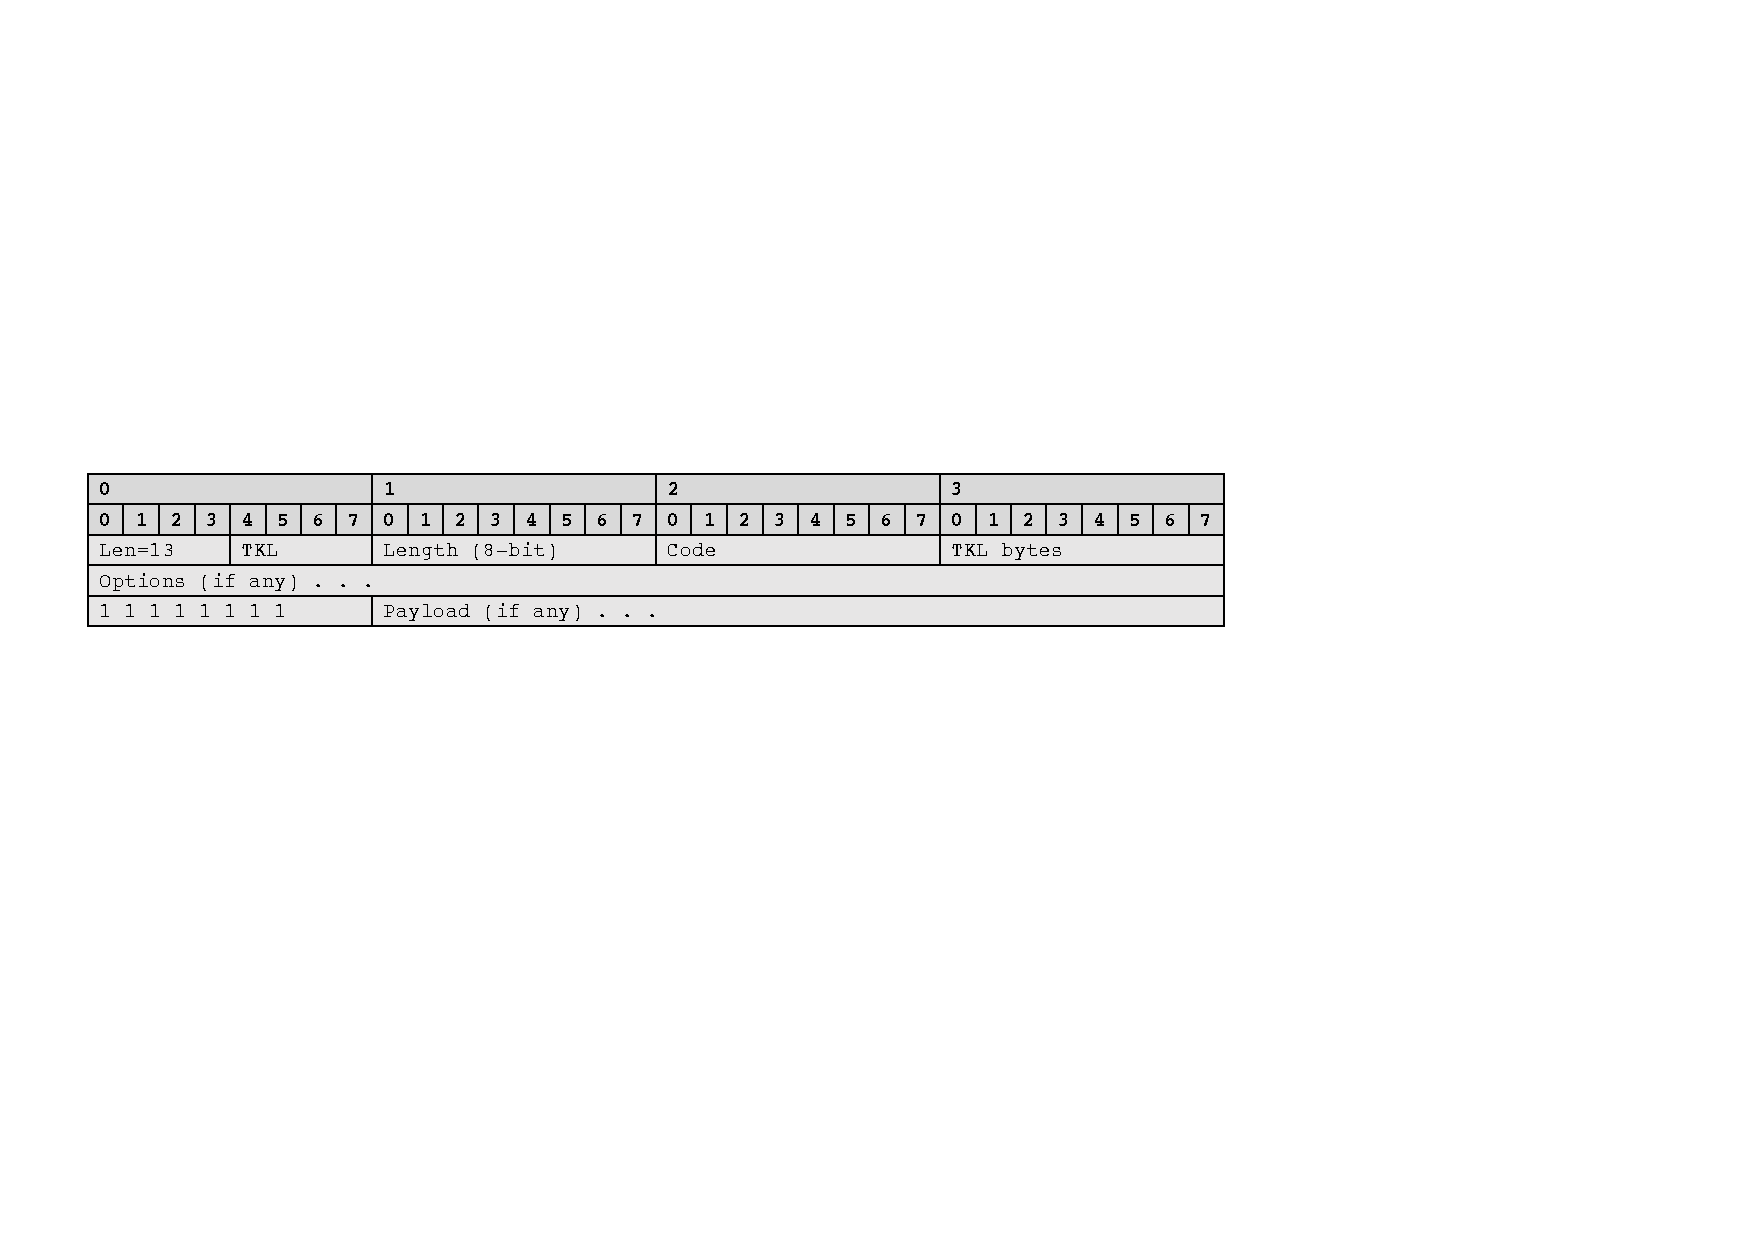
\includegraphics[width=3.5in]{gfx/msgformat-coapovertcp}
	\caption{The CoAP over TCP message format with 8-bit Length in header.}
	\label{fig:msgformatcoapovertcp}
\end{figure}

These fields are, Len and Length, which are used to indicate information about the amount of data sent in form of payload/options.  
This addition was necessary to take advantage of message delimitation supported by TCP.

%The use of TCP as a transport layer also makes it easier to avoid being blocked by firewalls.  
%The use of TCP as a transport layer also enables asynchronous message exchange, which makes it possible to transmit TCP requests simultaneously without the need for waiting for an acknowledgement. 

%TLS
%
%TCP has less risk of being blocked by firewalls than UDP
%No lost packages/data
%Provides additional information about session life to NAT
%Long lifetime
%No need for handling reliability
%(Exchanges messages asynchronously even though it runs TCP)
%TLS
%Is the changes in the header compatible with the current CoAP implementation?
%
%
%Background: Beskrivelse af de to protokoller, forholdsvis kort (undlade detaljer, som ikke er relevant for artiklen)





%\subsection{Middleware as Solution for Interoperability}
%Middleware has proven to be a solution in many environments for ensuring interoperability within distributed systems. In IoT the same way of thinking has been adapted. 
%Several projects in collaboration between big companies are currently developing  middleware solutions for IoT and one of these solutions is IoTivity which supports CoAP as an application protocol.
% 
%In \cite{interoperabilityChallenge} the IoTivity framework is evaluated according to defined requirements among others the connectivity where different connectivity models are evaluated. These connectivity models are device-to-device, device-to-gateway, and device-to-cloud. Results from the evaluation of IoTivity shows that device-to-cloud communication within constrained devices is challenging.
%
%\subsection{Device-to-Cloud}
%Existing solutions for communicating with device-to-cloud are HTTP, MQTT, CoAP...etc.
%
%compare solutions....
%
%
%HTTP 
%
%MQTT




\section{Related Work}
A great amount of work has been done in comparing the transport protocols, TCP and UDP. 

In \cite{giannoulis2009tcp} a performance evaluation of TCP and UDP is done on wireless multihop networks. The results of the evaluation shows clearly that TCP is a more power consuming protocol than UDP. Moreover it shows that UDP is faster and can send more data packets than TCP.

%These comparisons all clearly shows that TCP is more secure than UDP  but at the same time that TCP has a bigger overhead and thereby is more consuming than UDP.

%comparison of Ligthweight protocols
Another area which is related is the comparison of  
Lightweight protocols are important for constrained environments, such one can save on the ressources. 


%Comparison of protocols is related work

%TCPvsUDP 
%TCPvsUDP in lightweight protocols



%	The comparison of lightweight communication protocols has received attention by recent literature work. In [11], Davis et al. reported on the performance comparison between MQTT- S [3], a specification of MQTT adapted to the characteristics of low-power WSN environment, and CoAP. Our previous work in [9] presented the comparison between CoAP and HTTP in WSNs and demonstrated how CoAP improves the performance of constrained devices such as sensors and actuators. In [12], high level features (such as messaging capabilities, security, reliability, availability of implementations...) of MQTT and Advanced Message Queuing Protocol (AMQP) are evaluated and compared. A similar approach has been followed in [13] in order to compare MQTT and HTTP features. All the aforementioned comparisons of application protocols have not considered the use of smartphone but have only been limited in using lightweight application protocols in sensors and actuators. To the best of our knowledge, smartphone platforms have only been considered in [10], where Vergara et al describe a preliminary experimental evaluation of MQTT against HTTP. The comparison shows that the use of MQTT in Android devices decreases the energy consumption compared to HTTP in location based applications. To the best of our knowledge, the comparison between CoAP and MQTT has only been addressed in [6]. The comparison shows that CoAP lead to a lower bandwidth utilization as a consequence of the use of UDP instead of TCP as transport protocol. However, the comparison only considers the case in which the two protocols run on constrained battery operated gateways. They do not consider neither sensors and actuators nor smartphones. . 


%\section{CoAP over UDP and CoAP over TCP}


\subsection{CoAP over UDP}
Subsection text here.

\subsection{CoAP over TCP}
Subsection text here.

%\subsection{Publish-Subscribe Broker for CoAP}






% needed in second column of first page if using \IEEEpubid
%\IEEEpubidadjcol

\subsubsection{Subsubsection Heading Here}
Subsubsection text here.

%\section{Qualitative Comparison}
Here goes the qualitative comparison.
\section{Quantitative Comparison}
Here goes the quantitative comparison.

\subsection{Experiment Setup}
The different setups of the experiments are all based on the IoTivity framework running on two Linux (Ubuntu) machines. These two machines are both wireless coupled to a local network via a router. The test case for the experiments is meant to represent a constrained device, acting as a client, updating the temperature on a cloud server with a specific interval of time. 

Linux is chosen to represent a constrained device as it is necessary to be able to easily monitor the communication from the client side of view.

Setup for CoAP over UDP as illustrated in \figurename \ref{fig:setupudp} uses two applications. A simple IoTivity client and server application both developed in C++ using CoAP over UDP as an application protocol.
\begin{figure}[!t]
	\centering
	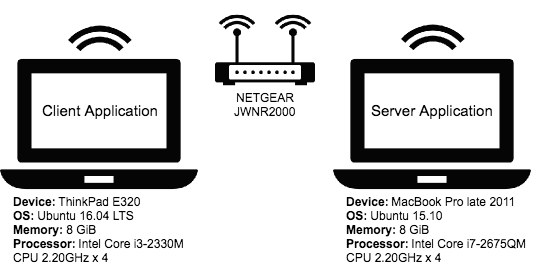
\includegraphics[width=3in]{gfx/setupa}
	\caption{Setup for CoAP over UDP.}
	\label{fig:setupudp}
\end{figure}

Setup for CoAP over TCP as illustrated in \figurename \ref{fig:setuptcp} uses two applications. A simple IoTivity client application developed in C++ and a simple IoTivity server application developed in Java. Both applications uses CoAP over TCP as an application protocol.
\begin{figure}[!t]
	\centering
	
\includegraphics[width=3in]{gfx/setupb}
	\caption{Setup for CoAP over TCP.}
	\label{fig:setuptcp}
\end{figure}

The memory consumption for the two client applications is presented in table \ref{tab:memory}:
%TABLE
The RAM measurements are done by using an AVR-tool called avr-size. The tool measures only the size of the initialized variables.
%Wireshark....
%\textbf{Memory consumption}\\
%Flyt den del til et afsnit med prototype implementation (før resultaterne)
%How much memory usage...

\subsection{Bandwidth}
In the following experiments the bandwidth of a \emph{single packet transaction} and the bandwidth of a \emph{complete communication scenario} for both aforementioned setups are measured. 
Bandwidth generated by communication protocols is directly related to the energy consumption. By measuring the bandwidth in bytes and multiplying it with the energy consumption of sending a single byte using Arduino Due, it is possible to calculate the complete energy consumption of the used constrained devices. 

\subsubsection{Single Packet Transaction}
This experiment is done where the client transmits a single packet, containing an arbitrary number, simulating a temperature measurement. \figurename{\ref{fig:singlepacket}} shows the results for a single packet transaction scenario, where CoAP (NON) and CoAP (CON) are the two different modes for CoAP over UDP. %CoAP (NON) is non-confirmable which means that the
\begin{figure}
	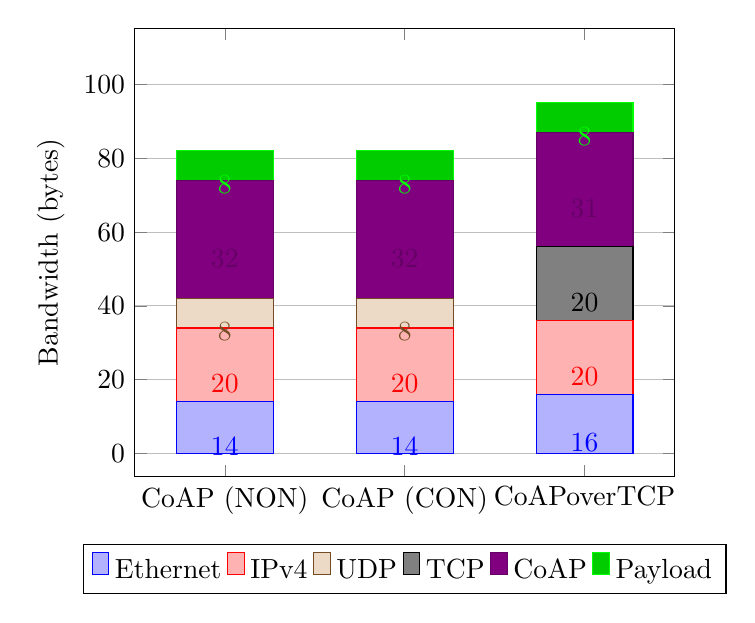
\begin{tikzpicture}
	\begin{axis}[
	%title={Single Packet Transaction (Client/Server)},
	ybar stacked,
	%ymax=50,
	ymajorgrids,
	bar width=35pt,
	%width=250pt,
	nodes near coords, 
	%nodes near coords={\pgfmathprintnumber\pgfplotspointmeta \%},
	nodes near coords align={anchor=north},%Move values in bar
	every node near coord/.style={
	},
	enlargelimits=0.25,
	legend style={at={(0.5,-0.15)},
		anchor=north,legend columns=-1},
	%width=0.8*\textwidth,
	ylabel={Bandwidth (bytes)},
	symbolic x coords={CoAP (NON), CoAP (CON), CoAPoverTCP},
	xtick=data,
	%legend pos= north east,
	%x tick label style={rotate=45,anchor=east},
	]
	%ethernet
	\addplot+[ybar] plot coordinates {(CoAP (NON),14) (CoAP (CON),14)
		(CoAPoverTCP,16) };
	%ipv4
	\addplot+[ybar] plot coordinates {(CoAP (NON),20) (CoAP (CON),20) 
		(CoAPoverTCP,20) };
	%udp
	\addplot+[ybar] plot coordinates {(CoAP (NON),8) (CoAP (CON),8) 
		(CoAPoverTCP,0) };
	%tcp
	\addplot+[ybar] plot coordinates {(CoAP (NON),0) (CoAP (CON),0) 
		(CoAPoverTCP,20) };
	%coap 
	\addplot+[ybar] plot coordinates {(CoAP (NON),32) (CoAP (CON),32) 
		(CoAPoverTCP,31) };
	%payload
	\addplot+[ybar] plot coordinates {(CoAP (NON),8) (CoAP (CON),8) 
		(CoAPoverTCP,8) };
	
	\legend{\strut Ethernet, \strut IPv4, \strut UDP, \strut TCP , \strut CoAP, \strut Payload}
	\end{axis}
	\end{tikzpicture}
	\caption{Single Packet Transaction (Client/Server).}
	\label{fig:singlepacket}
\end{figure}
It can be observed that CoAP over TCP overall has a lager packet than CoAP over UDP. This is primarily because of the TCP layer which has a 12 byte bigger overhead than UDP.
Though the CoAP layer in the CoAP over TCP packet is 1 byte shorter than CoAP over UDP, because of the MessageID-field (2 byte) is removed and replaced with the Length-field (1 byte).
%Why is ethernet 16 bytes???

With help of the measurements the energy consumption is calculated for the three packets. The calculation is shown below:
%calculation...

%TCP minimum header size is 20 bytes, but because of using options among others timestamp option, it is measured to 32 bytes. Timestamp option is enabled par default on Ubuntu 16.10.

\subsubsection{Complete Communication Scenario}
This experiment is done where the client transmits randomly generated numbers with an interval of 30 seconds, simulating temperature measurements, for a timespan of 30 minutes.
It is a complete scenario because the whole communication scenario, from it is initialised until it is terminated, is captured. The caption includes both the transmitted and the received packets.

\figurename{\ref{fig:completescenario}} shows the results for a complete scenario, where CoAP (NON) is omitted as it is not comparable with the two reliable CoAP versions, CoAP (CON) and CoAP over TCP. 
\begin{figure}[bht]
	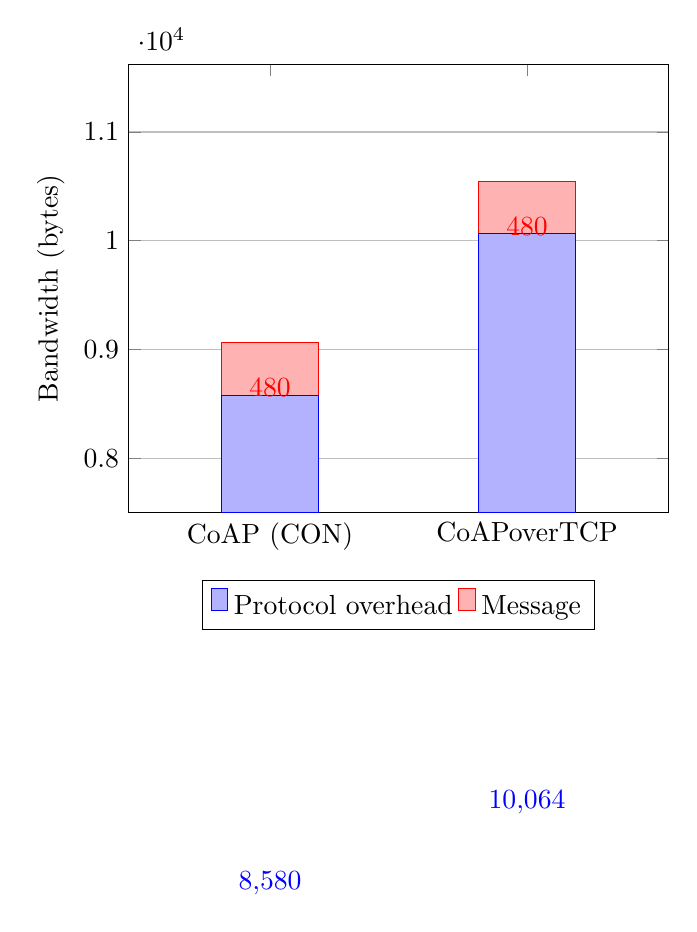
\begin{tikzpicture}
	\begin{axis}[
	%title={A complete communication scenario},
	ybar stacked,
	%ymax=50,
	ymajorgrids,
	bar width=35pt,
	%width=250pt,
	nodes near coords, 
	%nodes near coords={\pgfmathprintnumber\pgfplotspointmeta \%},
	nodes near coords align={anchor=north},%Move values in bar
	every node near coord/.style={
	},
	enlargelimits=0.55,
	legend style={at={(0.5,-0.15)},
		anchor=north,legend columns=-1},
	%width=0.8*\textwidth,
	ylabel={Bandwidth (bytes)},
	symbolic x coords={CoAP (CON), CoAPoverTCP},
	xtick=data,
	%legend pos= north east,
	%x tick label style={rotate=45,anchor=east},
	]
	%protocol overhead
	\addplot+[ybar] plot coordinates { (CoAP (CON),8580) 
		(CoAPoverTCP,10064) };
	%message
	\addplot+[ybar] plot coordinates { (CoAP (CON),480) 
		(CoAPoverTCP,480) };
	
	\legend{\strut Protocol overhead, \strut Message}
	\end{axis}
	\end{tikzpicture}
	\caption{A complete communication scenario.}
	\label{fig:completescenario}
\end{figure}

It is clear from the results that CoAP over TCP has a significantly larger overhead than CoAP (CON).
 
With help of the measurements the energy consumption is calculated for the two scenarios. The calculation is shown below:
%calculation...
%\textbf{En god ide er at maale energiforbruge / beregne det i joule. Giver et konkret svar om den kan bruges i specifikke typer af constraint devices}

\subsection{Latency}
In the following experiments the latency (RTT) is measured for the two setups in two scenarios, one with a noiseless channel and the other with a simulated noisy channel. The latency has an impact on the energy consumption. A long latency means less sleeping time which is a crucial element for a constrained to be able to save energy.
The noisy channel is emulated using the NetEM tool which provides Network Emulation functionality for testing protocols \cite{netem19:online}. 

These experiments are all done where the client transmits a total number of 60 transmissions. The RTT is calculated from the time a packet is sent until it receives the associated acknowledgement.

%Measure RTT values %which is the time from sending a package to receiving the acknowledgement.
%More latency = less time to sleep = more energy consumption
%Spredning/fordeling/varians af delay variations 

On \figurename{\ref{fig:coapconlatency}} and \figurename{\ref{fig:coaptcplatency}} the results of the first scenario with a noiseless channel for the respectively CoAP over UDP and CoAP over TCP setup are plotted into a histogram. 
\begin{figure}[bht]
	\centering
	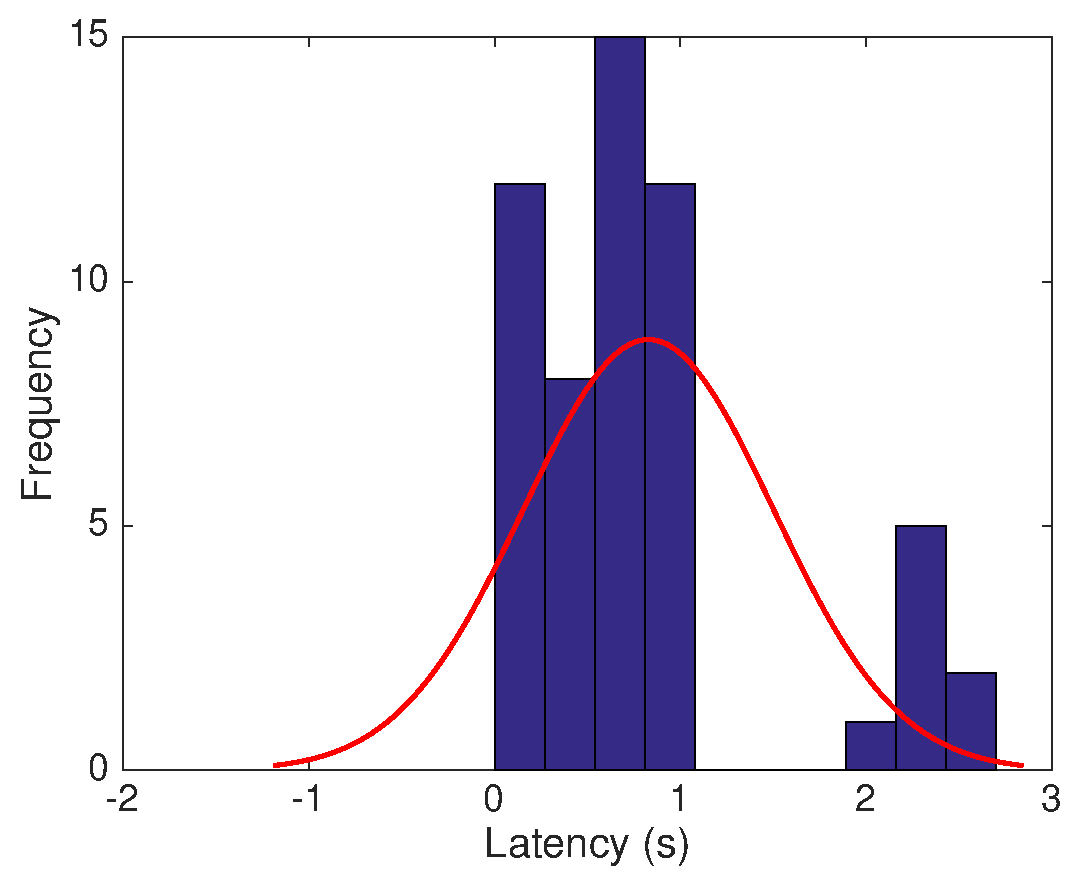
\includegraphics[width=3in]{gfx/coapoverudp}
	\caption{Latency for CoAP over UDP in a noiseless channel.}
	\label{fig:coapconlatency}
\end{figure}
\begin{figure}[bht]
	\centering
	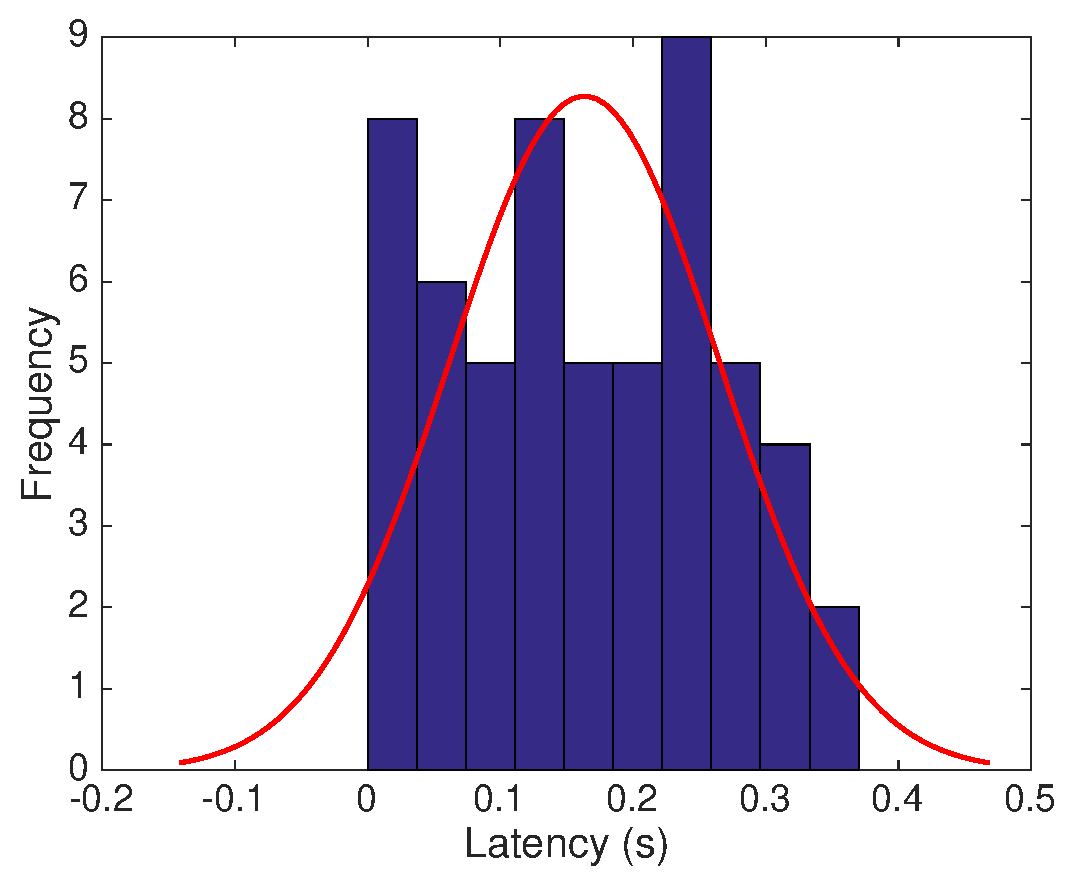
\includegraphics[width=3in]{gfx/coapovertcp}
	\caption{Latency for CoAP over TCP in a noiseless channel.}
	\label{fig:coaptcplatency}
\end{figure}


%TCP direct from transport layer therefore faster
%UDP from application layer therefore slower


%More lost packet = more packet to send = more energy consumption
This is the \figurename \ref{coapovertcploss}
\begin{figure}[bh]
	\centering
	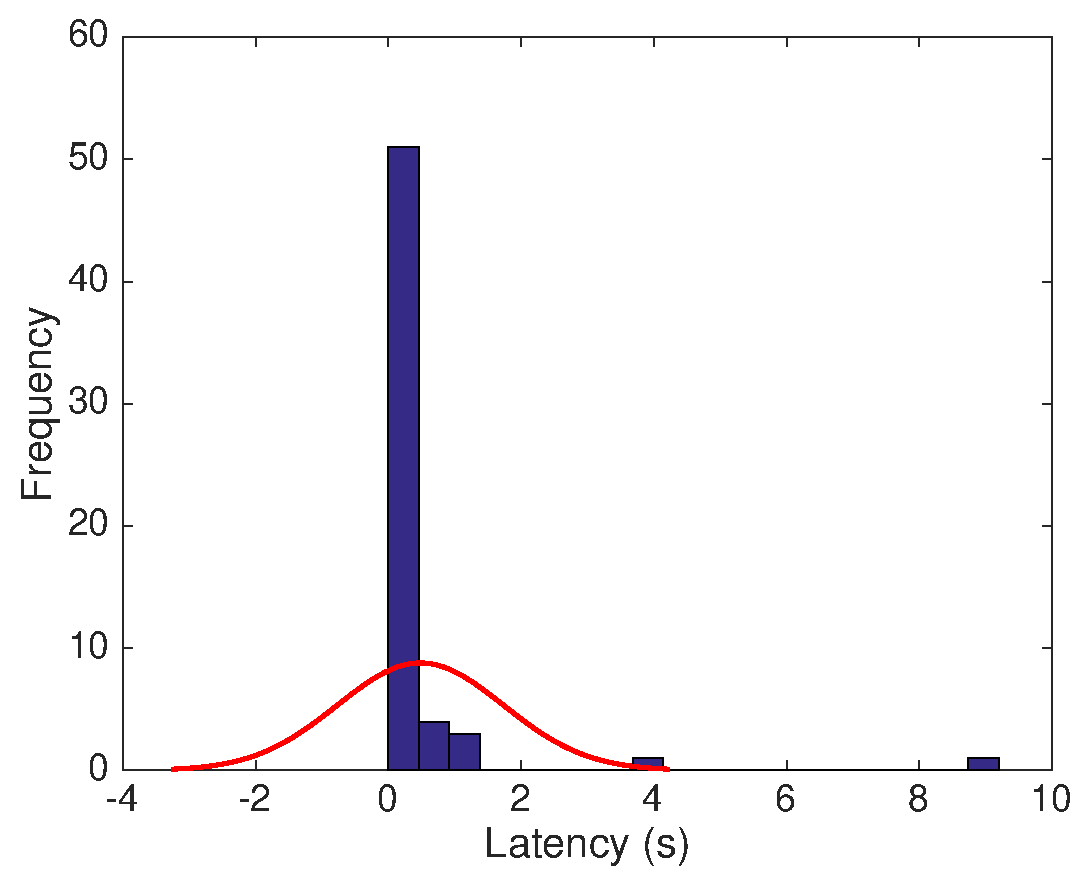
\includegraphics[width=3in]{gfx/coapovertcp25loss}
	\caption{Latency for CoAP over TCP with 25 \% packet loss.}
	\label{coapovertcploss}
\end{figure}

This is the \figurename \ref{coapoverudploss}
\begin{figure}[bh]
	\centering
	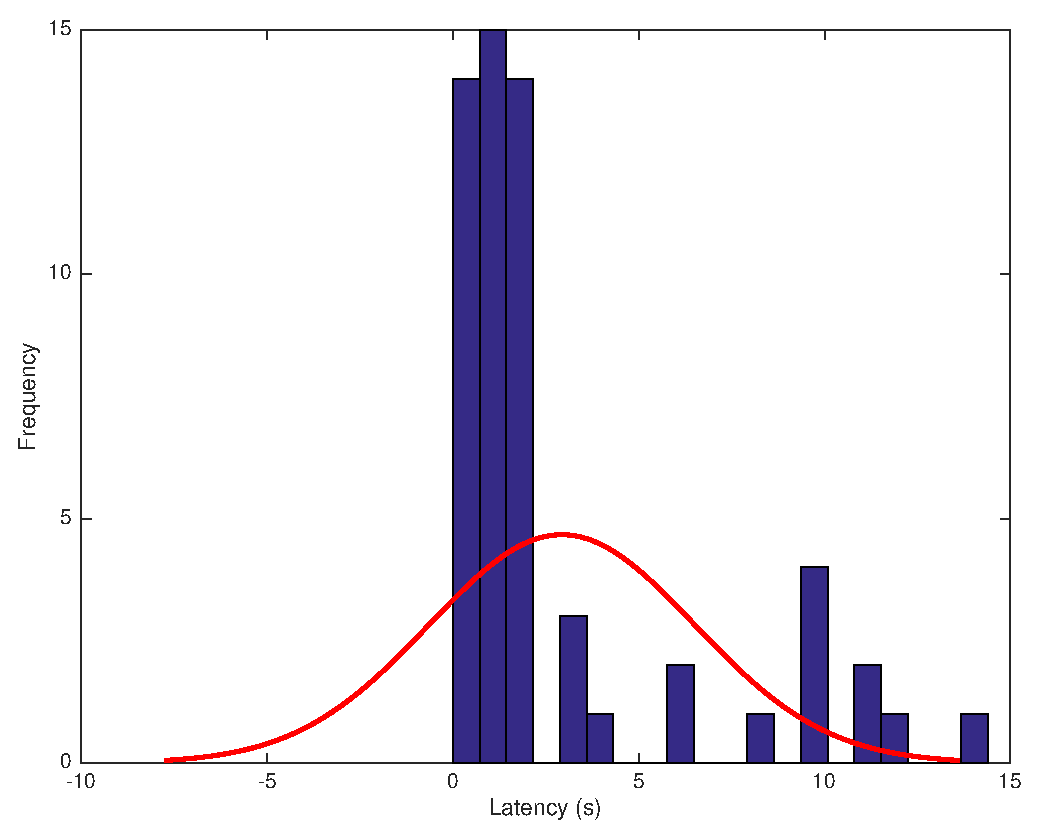
\includegraphics[width=3in]{gfx/coapoverudp25loss}
	\caption{Latency for CON CoAP with 25 \% packet loss.}
	\label{coapoverudploss}
\end{figure}


\section{Discussion}\label{sec:discussion}
The purpose of the comparison is to evaluate if it is advantageous to use TCP as a transport protocol in CoAP instead of UDP, when CoAP is used for constrained IoT devices. 

%Energy measurements  ---> case study
The calculations in the case study, which are based on the experimental results, show that CoAP over TCP consumes less power than regular CoAP. Therefore the calculations in the case study also shows that CoAP over TCP, if used in Arduino Due, will give a better lifetime than regular CoAP. 
It is clear from the results that the bandwidth does not have a big influence on the overall energy consumption even though the results of the bandwidth experiments show that the bandwidth for CoAP over TCP is higher than the bandwidth for regular CoAP, for both the single packet transaction scenario and the complete communication scenario. 
%This was expected as previous work has shown that TCP is more power consuming, which is most likely caused by the bandwidth. 
%The case study shows that in both versions of CoAP the energy consumption is very low making the difference near insignificant. However, it is also shown in the case study that for a longer timespan the difference in energy consumption is very significant, unlike the scenario with a short timespan. 

Latency has much more effect on the results for energy consumption, as it prevents the constrained device to be in power-saving mode while waiting for an acknowledgement. 
The reason to why TCP performs good in the latency results is due to a persistent connection. 
On the other hand, if TCP is used in a not-persistent connection it will have a much worse latency \cite{ludovici2013tinycoap}. But still the results, showing that CoAP has a bad latency performance compared to CoAP over TCP, are unexpected.
The fact that CoAP sends acknowledgement using the application layer, whereas CoAP over TCP sends acknowledgement already from the transport layer, has an impact, but not enough to explain the big difference in the results. 
In \cite{hayden1997optimizing} it is observed that overheads for crossing layers in different systems can be up to 50 \textmu s, which is a very insignificant number compared with the results in the experiments.
%handshake tcp

To confirm the results of the latency experiment with CoAP, a similar experiment with a total of 20 transmissions are made, using Californium \cite{Calif82:online}, which is another CoAP implementation, made in Java. The results give an average latency of 15.22 ms against 813.15 ms. 
A big difference is observed in the different measurements, confirming that the CoAP protocol is able to achieve a much better latency performance depending on the implementation. It is unknown, why IoTivity compared to Californium, has a poor latency performance.
It can be concluded from the results of the experiments made using the IoTivity implementations of CoAP and CoAP over TCP, that from an energy perspective, it is advantageous to use TCP as a transport protocol in CoAP instead of UDP.
There is however, a single case where CoAP is advantagous to use, and this is when memory is in focus, because CoAP over TCP will probably be more memory consuming than CoAP.  

%On the other hand the results of the latency experiments shows that CoAP over TCP has a much better latency than regular CoAP in both a noiseless channel and in a noisy channel. 
%These results tells that using TCP as a transport layer for CoAP  is preferable in specific cases, even though it has a higher bandwidth than regular CoAP. 
%Such a case could for example be a constrained device which often has to collect data about the temperature for use in e.g. a weather application. Frequent data collection needs short delays to obtain better results and therefore CoAP over TCP is more suitable for this case. This device can however not be battery driven due to the energy calculation done in section \ref{sec:casestudy}. This constrained device should also have a sufficient amount of memory to be able to cope with the extra overhead as a result of using TCP/IP stack implementation. 
%These results however tells that using UDP as a transport layer for CoAP is preferable in cases with very constrained devices, specially for battery driven devices and for devices that has a very tight memory space. An example for such a case is .... ??????? 



%It is clearly from the results that it is advantageous to use TCP as a transport protocol in CoAP instead of UDP.
%
%From the results it is shown that the bandwidth for CoAP over TCP is higher than the bandwidth for regular CoAP.
%
%On the other side regular CoAP over TCP has a much better latency than regular CoAP.

% UDP vs TCP - A mixed solution between TCP and UDP


% BANDWIDTH
	% CALCULATIONS
	
% LATENCY

% CASES



% MEMORY



% An example of a floating figure using the graphicx package.
% Note that \label must occur AFTER (or within) \caption.
% For figures, \caption should occur after the \includegraphics.
% Note that IEEEtran v1.7 and later has special internal code that
% is designed to preserve the operation of \label within \caption
% even when the captionsoff option is in effect. However, because
% of issues like this, it may be the safest practice to put all your
% \label just after \caption rather than within \caption{}.
%
% Reminder: the "draftcls" or "draftclsnofoot", not "draft", class
% option should be used if it is desired that the figures are to be
% displayed while in draft mode.
%
%\begin{figure}[!t]
%\centering
%\includegraphics[width=2.5in]{myfigure}
% where an .eps filename suffix will be assumed under latex, 
% and a .pdf suffix will be assumed for pdflatex; or what has been declared
% via \DeclareGraphicsExtensions.
%\caption{Simulation results for the network.}
%\label{fig_sim}
%\end{figure}

% Note that the IEEE typically puts floats only at the top, even when this
% results in a large percentage of a column being occupied by floats.


% An example of a double column floating figure using two subfigures.
% (The subfig.sty package must be loaded for this to work.)
% The subfigure \label commands are set within each subfloat command,
% and the \label for the overall figure must come after \caption.
% \hfil is used as a separator to get equal spacing.
% Watch out that the combined width of all the subfigures on a 
% line do not exceed the text width or a line break will occur.
%
%\begin{figure*}[!t]
%\centering
%\subfloat[Case I]{\includegraphics[width=2.5in]{box}%
%\label{fig_first_case}}
%\hfil
%\subfloat[Case II]{\includegraphics[width=2.5in]{box}%
%\label{fig_second_case}}
%\caption{Simulation results for the network.}
%\label{fig_sim}
%\end{figure*}
%
% Note that often IEEE papers with subfigures do not employ subfigure
% captions (using the optional argument to \subfloat[]), but instead will
% reference/describe all of them (a), (b), etc., within the main caption.
% Be aware that for subfig.sty to generate the (a), (b), etc., subfigure
% labels, the optional argument to \subfloat must be present. If a
% subcaption is not desired, just leave its contents blank,
% e.g., \subfloat[].


% An example of a floating table. Note that, for IEEE style tables, the
% \caption command should come BEFORE the table and, given that table
% captions serve much like titles, are usually capitalized except for words
% such as a, an, and, as, at, but, by, for, in, nor, of, on, or, the, to
% and up, which are usually not capitalized unless they are the first or
% last word of the caption. Table text will default to \footnotesize as
% the IEEE normally uses this smaller font for tables.
% The \label must come after \caption as always.
%
%\begin{table}[!t]
%% increase table row spacing, adjust to taste
%\renewcommand{\arraystretch}{1.3}
% if using array.sty, it might be a good idea to tweak the value of
% \extrarowheight as needed to properly center the text within the cells
%\caption{An Example of a Table}
%\label{table_example}
%\centering
%% Some packages, such as MDW tools, offer better commands for making tables
%% than the plain LaTeX2e tabular which is used here.
%\begin{tabular}{|c||c|}
%\hline
%One & Two\\
%\hline
%Three & Four\\
%\hline
%\end{tabular}
%\end{table}


% Note that the IEEE does not put floats in the very first column
% - or typically anywhere on the first page for that matter. Also,
% in-text middle ("here") positioning is typically not used, but it
% is allowed and encouraged for Computer Society conferences (but
% not Computer Society journals). Most IEEE journals/conferences use
% top floats exclusively. 
% Note that, LaTeX2e, unlike IEEE journals/conferences, places
% footnotes above bottom floats. This can be corrected via the
% \fnbelowfloat command of the stfloats package.




%\section{Conclusion}
\section{Conclusion}
%Conclusion and Futurework
The conclusion goes here.





% if have a single appendix:
%\appendix[Proof of the Zonklar Equations]
% or
%\appendix  % for no appendix heading
% do not use \section anymore after \appendix, only \section*
% is possibly needed

% use appendices with more than one appendix
% then use \section to start each appendix
% you must declare a \section before using any
% \subsection or using \label (\appendices by itself
% starts a section numbered zero.)
%


%\appendices
%\section{Proof of the First Zonklar Equation}
%Appendix one text goes here.

% you can choose not to have a title for an appendix
% if you want by leaving the argument blank
%\section{}
%Appendix two text goes here.


% use section* for acknowledgment
\section*{Acknowledgment}


The authors would like to thank...


% Can use something like this to put references on a page
% by themselves when using endfloat and the captionsoff option.
\ifCLASSOPTIONcaptionsoff
  \newpage
\fi



% trigger a \newpage just before the given reference
% number - used to balance the columns on the last page
% adjust value as needed - may need to be readjusted if
% the document is modified later
%\IEEEtriggeratref{8}
% The "triggered" command can be changed if desired:
%\IEEEtriggercmd{\enlargethispage{-5in}}


% references section
%% can use a bibliography generated by BibTeX as a .bbl file
% BibTeX documentation can be easily obtained at:
% http://mirror.ctan.org/biblio/bibtex/contrib/doc/
% The IEEEtran BibTeX style support page is at:
% http://www.michaelshell.org/tex/ieeetran/bibtex/
%\bibliographystyle{IEEEtran}
% argument is your BibTeX string definitions and bibliography database(s)
%\bibliography{IEEEabrv,../bib/paper}
%
% <OR> manually copy in the resultant .bbl file
% set second argument of \begin to the number of references
% (used to reserve space for the reference number labels box)
%\begin{thebibliography}{1}
%********************************************************************
% Bibliographies
%*******************************************************


%\addbibresource{IEEEexample.bib}
%\addbibresource[label=ownpubs]{AMiede_Publications.bib}



%\bibitem{interoperabilityChallenge}
%H.~Kopka and P.~W. Daly, \emph{A Guide to \LaTeX}, 3rd~ed.\hskip 1em plus
%0.5em minus 0.4em\relax Harlow, England: Addison-Wesley, 1999.

%\bibitem{IEEEhowto:kopka}
%H.~Kopka and P.~W. Daly, \emph{A Guide to \LaTeX}, 3rd~ed.\hskip 1em plus
%0.5em minus 0.4em\relax Harlow, England: Addison-Wesley, 1999.


%\end{thebibliography}

% biography section
% 
% If you have an EPS/PDF photo (graphicx package needed) extra braces are
% needed around the contents of the optional argument to biography to prevent
% the LaTeX parser from getting confused when it sees the complicated
% \includegraphics command within an optional argument. (You could create
% your own custom macro containing the \includegraphics command to make things
% simpler here.)
%\begin{IEEEbiography}[{\includegraphics[width=1in,height=1.25in,clip,keepaspectratio]{mshell}}]{Michael Shell}
% or if you just want to reserve a space for a photo:




% insert where needed to balance the two columns on the last page with
% biographies
%\newpage


% You can push biographies down or up by placing
% a \vfill before or after them. The appropriate
% use of \vfill depends on what kind of text is
% on the last page and whether or not the columns
% are being equalized.

%\vfill

% Can be used to pull up biographies so that the bottom of the last one
% is flush with the other column.
%\enlargethispage{-5in}

%********************************************************************
% Bibliographies
%*******************************************************
\nocite{*}
\bibliographystyle{IEEEtran}
\bibliography{IEEEabrv,Bibliography}

% that's all folks
\end{document}


